\documentclass[portrait,a4, final]{baposter}

\tracingstats=2

\usepackage{times}
\usepackage{calc}
\usepackage{graphicx}
\usepackage{amsmath}
\usepackage{amssymb}
\usepackage{relsize}
\usepackage{multirow}
\usepackage{bm}

\usepackage{graphicx}
\usepackage{multicol}
\usepackage{wrapfig}

\usepackage{pgfbaselayers}
\pgfdeclarelayer{background}
\pgfdeclarelayer{foreground}
\pgfsetlayers{background,main,foreground}

\usepackage{helvet}
%\usepackage{bookman}
\usepackage{palatino}

\usepackage{booktabs}% http://ctan.org/pkg/booktabs


\newcommand{\captionfont}{\footnotesize}

\selectcolormodel{rgb}

\graphicspath{{images/}}

%%%%%%%%%%%%%%%%%%%%%%%%%%%%%%%%%%%%%%%%%%%%%%%%%%%%%%%%%%%%%%%%%%%%%%%%%%%%%%%%
%%%% Some math symbols used in the text
%%%%%%%%%%%%%%%%%%%%%%%%%%%%%%%%%%%%%%%%%%%%%%%%%%%%%%%%%%%%%%%%%%%%%%%%%%%%%%%%
% Format 
\newcommand{\Matrix}[1]{\begin{bmatrix} #1 \end{bmatrix}}
\newcommand{\Vector}[1]{\Matrix{#1}}
\newcommand*{\SET}[1]  {\ensuremath{\mathcal{#1}}}
\newcommand*{\MAT}[1]  {\ensuremath{\mathbf{#1}}}
\newcommand*{\VEC}[1]  {\ensuremath{\bm{#1}}}
\newcommand*{\CONST}[1]{\ensuremath{\mathit{#1}}}
\newcommand*{\norm}[1]{\mathopen\| #1 \mathclose\|}% use instead of $\|x\|$
\newcommand*{\abs}[1]{\mathopen| #1 \mathclose|}% use instead of $\|x\|$
\newcommand*{\absLR}[1]{\left| #1 \right|}% use instead of $\|x\|$

\def\norm#1{\mathopen\| #1 \mathclose\|}% use instead of $\|x\|$
\newcommand{\normLR}[1]{\left\| #1 \right\|}% use instead of $\|x\|$

%%%%%%%%%%%%%%%%%%%%%%%%%%%%%%%%%%%%%%%%%%%%%%%%%%%%%%%%%%%%%%%%%%%%%%%%%%%%%%%%
% Multicol Settings
%%%%%%%%%%%%%%%%%%%%%%%%%%%%%%%%%%%%%%%%%%%%%%%%%%%%%%%%%%%%%%%%%%%%%%%%%%%%%%%%
\setlength{\columnsep}{0.7em}
\setlength{\columnseprule}{0mm}


%%%%%%%%%%%%%%%%%%%%%%%%%%%%%%%%%%%%%%%%%%%%%%%%%%%%%%%%%%%%%%%%%%%%%%%%%%%%%%%%
% Save space in lists. Use this after the opening of the list
%%%%%%%%%%%%%%%%%%%%%%%%%%%%%%%%%%%%%%%%%%%%%%%%%%%%%%%%%%%%%%%%%%%%%%%%%%%%%%%%
\newcommand{\compresslist}{%
\setlength{\itemsep}{1pt}%
\setlength{\parskip}{0pt}%
\setlength{\parsep}{0pt}%
}


%%%%%%%%%%%%%%%%%%%%%%%%%%%%%%%%%%%%%%%%%%%%%%%%%%%%%%%%%%%%%%%%%%%%%%%%%%%%%%
%%% Begin of Document
%%%%%%%%%%%%%%%%%%%%%%%%%%%%%%%%%%%%%%%%%%%%%%%%%%%%%%%%%%%%%%%%%%%%%%%%%%%%%%

\begin{document}

%%%%%%%%%%%%%%%%%%%%%%%%%%%%%%%%%%%%%%%%%%%%%%%%%%%%%%%%%%%%%%%%%%%%%%%%%%%%%%
%%% Here starts the poster
%%%---------------------------------------------------------------------------
%%% Format it to your taste with the options
%%%%%%%%%%%%%%%%%%%%%%%%%%%%%%%%%%%%%%%%%%%%%%%%%%%%%%%%%%%%%%%%%%%%%%%%%%%%%%
% Define some colors
%\definecolor{silver}{cmyk}{0,0,0,0.3}
%\definecolor{yellow}{cmyk}{0,0,0.9,0.0}
%\definecolor{reddishyellow}{cmyk}{0,0.22,1.0,0.0}
%\definecolor{black}{cmyk}{0,0,0.0,1.0}
%\definecolor{darkYellow}{cmyk}{0,0,1.0,0.5}
%\definecolor{darkSilver}{cmyk}{0,0,0,0.1}

%\definecolor{lightyellow}{cmyk}{0,0,0.3,0.0}
%\definecolor{lighteryellow}{cmyk}{0,0,0.1,0.0}
%\definecolor{lighteryellow}{cmyk}{0,0,0.1,0.0}
%\definecolor{lightestyellow}{cmyk}{0,0,0.05,0.0}

\definecolor{black}{rgb}{0,0,0}
\definecolor{white}{rgb}{255,255,255}

% SU_blue
% \definecolor{SU_blue}{rgb}{0.000000,0.184314,0.372549}
\definecolor{SU_blue}{rgb}{0.098039, 0.329411,0.729411}
\definecolor{SU_blue80}{rgb}{0.000000,0.147451,0.298039}
\definecolor{SU_blue60}{rgb}{0.000000,0.110588,0.223529}
\definecolor{SU_blue40}{rgb}{0.000000,0.073725,0.149020}
\definecolor{SU_blue20}{rgb}{0.000000,0.036863,0.074510}
% SU_olive
\definecolor{SU_olive}{rgb}{0.639216,0.658824,0.419608}
\definecolor{SU_olive80}{rgb}{0.511373,0.527059,0.335686}
\definecolor{SU_olive60}{rgb}{0.383529,0.395294,0.251765}
\definecolor{SU_olive40}{rgb}{0.255686,0.263529,0.167843}
\definecolor{SU_olive20}{rgb}{0.127843,0.131765,0.083922}
% SU_sky
\definecolor{SU_sky}{rgb}{0.674510,0.870588,0.901961}
\definecolor{SU_sky80}{rgb}{0.539608,0.696471,0.721569}
\definecolor{SU_sky60}{rgb}{0.404706,0.522353,0.541176}
\definecolor{SU_sky40}{rgb}{0.269804,0.348235,0.360784}
\definecolor{SU_sky20}{rgb}{0.134902,0.174118,0.180392}
% SU_water
\definecolor{SU_water}{rgb}{0.607843,0.698039,0.807843}
\definecolor{SU_water80}{rgb}{0.486275,0.558431,0.646275}
\definecolor{SU_water60}{rgb}{0.364706,0.418824,0.484706}
\definecolor{SU_water40}{rgb}{0.243137,0.279216,0.323137}
\definecolor{SU_water20}{rgb}{0.121569,0.139608,0.161569}
% SU_fire
\definecolor{SU_fire}{rgb}{0.850980,0.368627,0.000000}
\definecolor{SU_fire80}{rgb}{0.680784,0.294902,0.000000}
\definecolor{SU_fire60}{rgb}{0.510588,0.221176,0.000000}
\definecolor{SU_fire40}{rgb}{0.340392,0.147451,0.000000}
\definecolor{SU_fire20}{rgb}{0.170196,0.073725,0.000000}
% SU_silver
\definecolor{SU_silver}{rgb}{0.737255,0.741176,0.737255}
\definecolor{SU_silver80}{rgb}{0.589804,0.592941,0.589804}
\definecolor{SU_silver60}{rgb}{0.442353,0.444706,0.442353}
\definecolor{SU_silver40}{rgb}{0.294902,0.296471,0.294902}
\definecolor{SU_silver20}{rgb}{0.147451,0.148235,0.147451}


%%
\typeout{Poster Starts}
\background{
  \begin{tikzpicture}[remember picture,overlay]%
    \draw (current page.north west)+(-2em,2em) node[anchor=north west] {\includegraphics[height=1.1\textheight]{silhouettes_background}};
  \end{tikzpicture}%
}

\newlength{\leftimgwidth}
\begin{poster}%
  % Poster Options
  {
  % Show grid to help with alignment
  grid=no,
  % Column spacing
  colspacing=1em,
  % Color style
  bgColorOne=white,
  bgColorTwo=SU_blue,
  borderColor=white,
  headerColorOne=SU_blue,
  headerColorTwo=SU_blue,
  headerFontColor=white,
  boxColorOne=white, %SU_sky,
  boxColorTwo=SU_sky,
  % Format of textbox
  textborder=roundedleft,
  % Format of text header
  eyecatcher=yes,
  headerborder=open,
  headerheight=0.08\textheight,
  headershape=roundedright,
  headershade=plain,
  headerfont=\Large\textsf, %Sans Serif
  boxshade=plain,
%  background=shade-tb,
  background=plain,
  linewidth=2pt
  }
  % Eye Catcher
  {
\includegraphics[height=5em]{Kth_logo2.png}} % No eye catcher for this poster. (eyecatcher=no above). If an eye catcher is present, the title is centered between eye-catcher and logo.
  % Title
  {\sf %Sans Serif
  %\bf% Serif
  \color{black} Learning sequence disambiguation with synaptic traces in associative neural networks}
  % Authors
  {\sf %Sans Serif
  % Serif
  \vspace{0.5em}
  \color{SU_fire} Ram{\'o}n Mart{\'i}nez\textsuperscript{1},  Anders Lansner\textsuperscript{1, 2}, Pawel Herman\textsuperscript{1}\\ 
  \color{black}
  \smaller{\smaller{\smaller{ 1) KTH, Royal Institute of Technology 2) Stockholm University, Mathematics and KTH Royal Institute of Technology}}}
  }
  % University logo
  {% The makebox allows the title to flow into the logo, this is a hack because of the L shaped logo.
    \makebox[10em][r]{%
      \begin{minipage}{16em}
        \hfill
        %\includegraphics[height=7.0em]{CERN_logo_white_on_transparent}
        \vspace{-10pt}
        
\includegraphics[height=6.0em]{euro_spin_logo.jpg}
      \end{minipage}
    }
  }

  \tikzstyle{light shaded}=[top color=baposterBGtwo!30!white,bottom color=baposterBGone!30!white,shading=axis,shading angle=30]

  % Width of left inset image
     \setlength{\leftimgwidth}{0.78em+8.0em}

%%%%%%%%%%%%%%%%%%%%%%%%%%%%%%%%%%%%%%%%%%%%%%%%%%%%%%%%%%%%%%%%%%%%%%%%%%%%%%
%%% Now define the boxes that make up the poster
%%%---------------------------------------------------------------------------
%%% Each box has a name and can be placed absolutely or relatively.
%%% The only inconvenience is that you can only specify a relative position 
%%% towards an already declared box. So if you have a box attached to the 
%%% bottom, one to the top and a third one which should be in between, you 
%%% have to specify the top and bottom boxes before you specify the middle 
%%% box.
%%%%%%%%%%%%%%%%%%%%%%%%%%%%%%%%%%%%%%%%%%%%%%%%%%%%%%%%%%%%%%%%%%%%%%%%%%%%%%
    %
    % A colored circle useful as a bullet with an adjustably strong filling
    \newcommand{\coloredcircle}[1]{%
      \tikz{\useasboundingbox (-0.2em,-0.32em) rectangle(0.2em,0.32em); \draw[draw=black,fill=SU_blue!80!black!#1!white,line width=0.03em] (0,0) circle(0.18em);}}

%%%%%%%%%%%%%%%%%%%%%%%%%%%%%%%%%%%%%%%%%%%%%%%%%%%%%%%%%%%%%%%%%%%%%%%%%%%%%%
  \headerbox{Sequence Learning}{name=sequences,column=0,row=0}{
%%%%%%%%%%%%%%%%%%%%%%%%%%%%%%%%%%%%%%%%%%%%%%%%%%%%%%%%%%%%%%%%%%%%%%%%%%%%%%
  Sequence disambiguation or using past context to determine the trajectory of a sequence has been deemed one of themost important problems that a sequence prediction network should solve \cite{levy}. There have been a few attempts at the problem of sequence disambiguation in the attractor network framework but most of them rely on non-local learning rules or require an unfeasible large number of parameter. We present here a sequence learning system that works with probabilistic associative learning and is able to accomplish sequence disambiguation by using dynamical information in the form of synaptic traces.}



%%%%%%%%%%%%%%%%%%%%%%%%%%%%%%%%%%%%%%%%%%%%%%%%%%%%%%%%%%%%%%%%%%%%%%%%%%%%%%
  \headerbox{Effects of noise}{name=noise,column=0,span=1,below=sequences}{
%%%%%%%%%%%%%%%%%%%%%%%%%%%%%%%%%%%%%%%%%%%%%%%%%%%%%%%%%%%%%%%%%%%%%%%%%%%%%%

\begin{center}
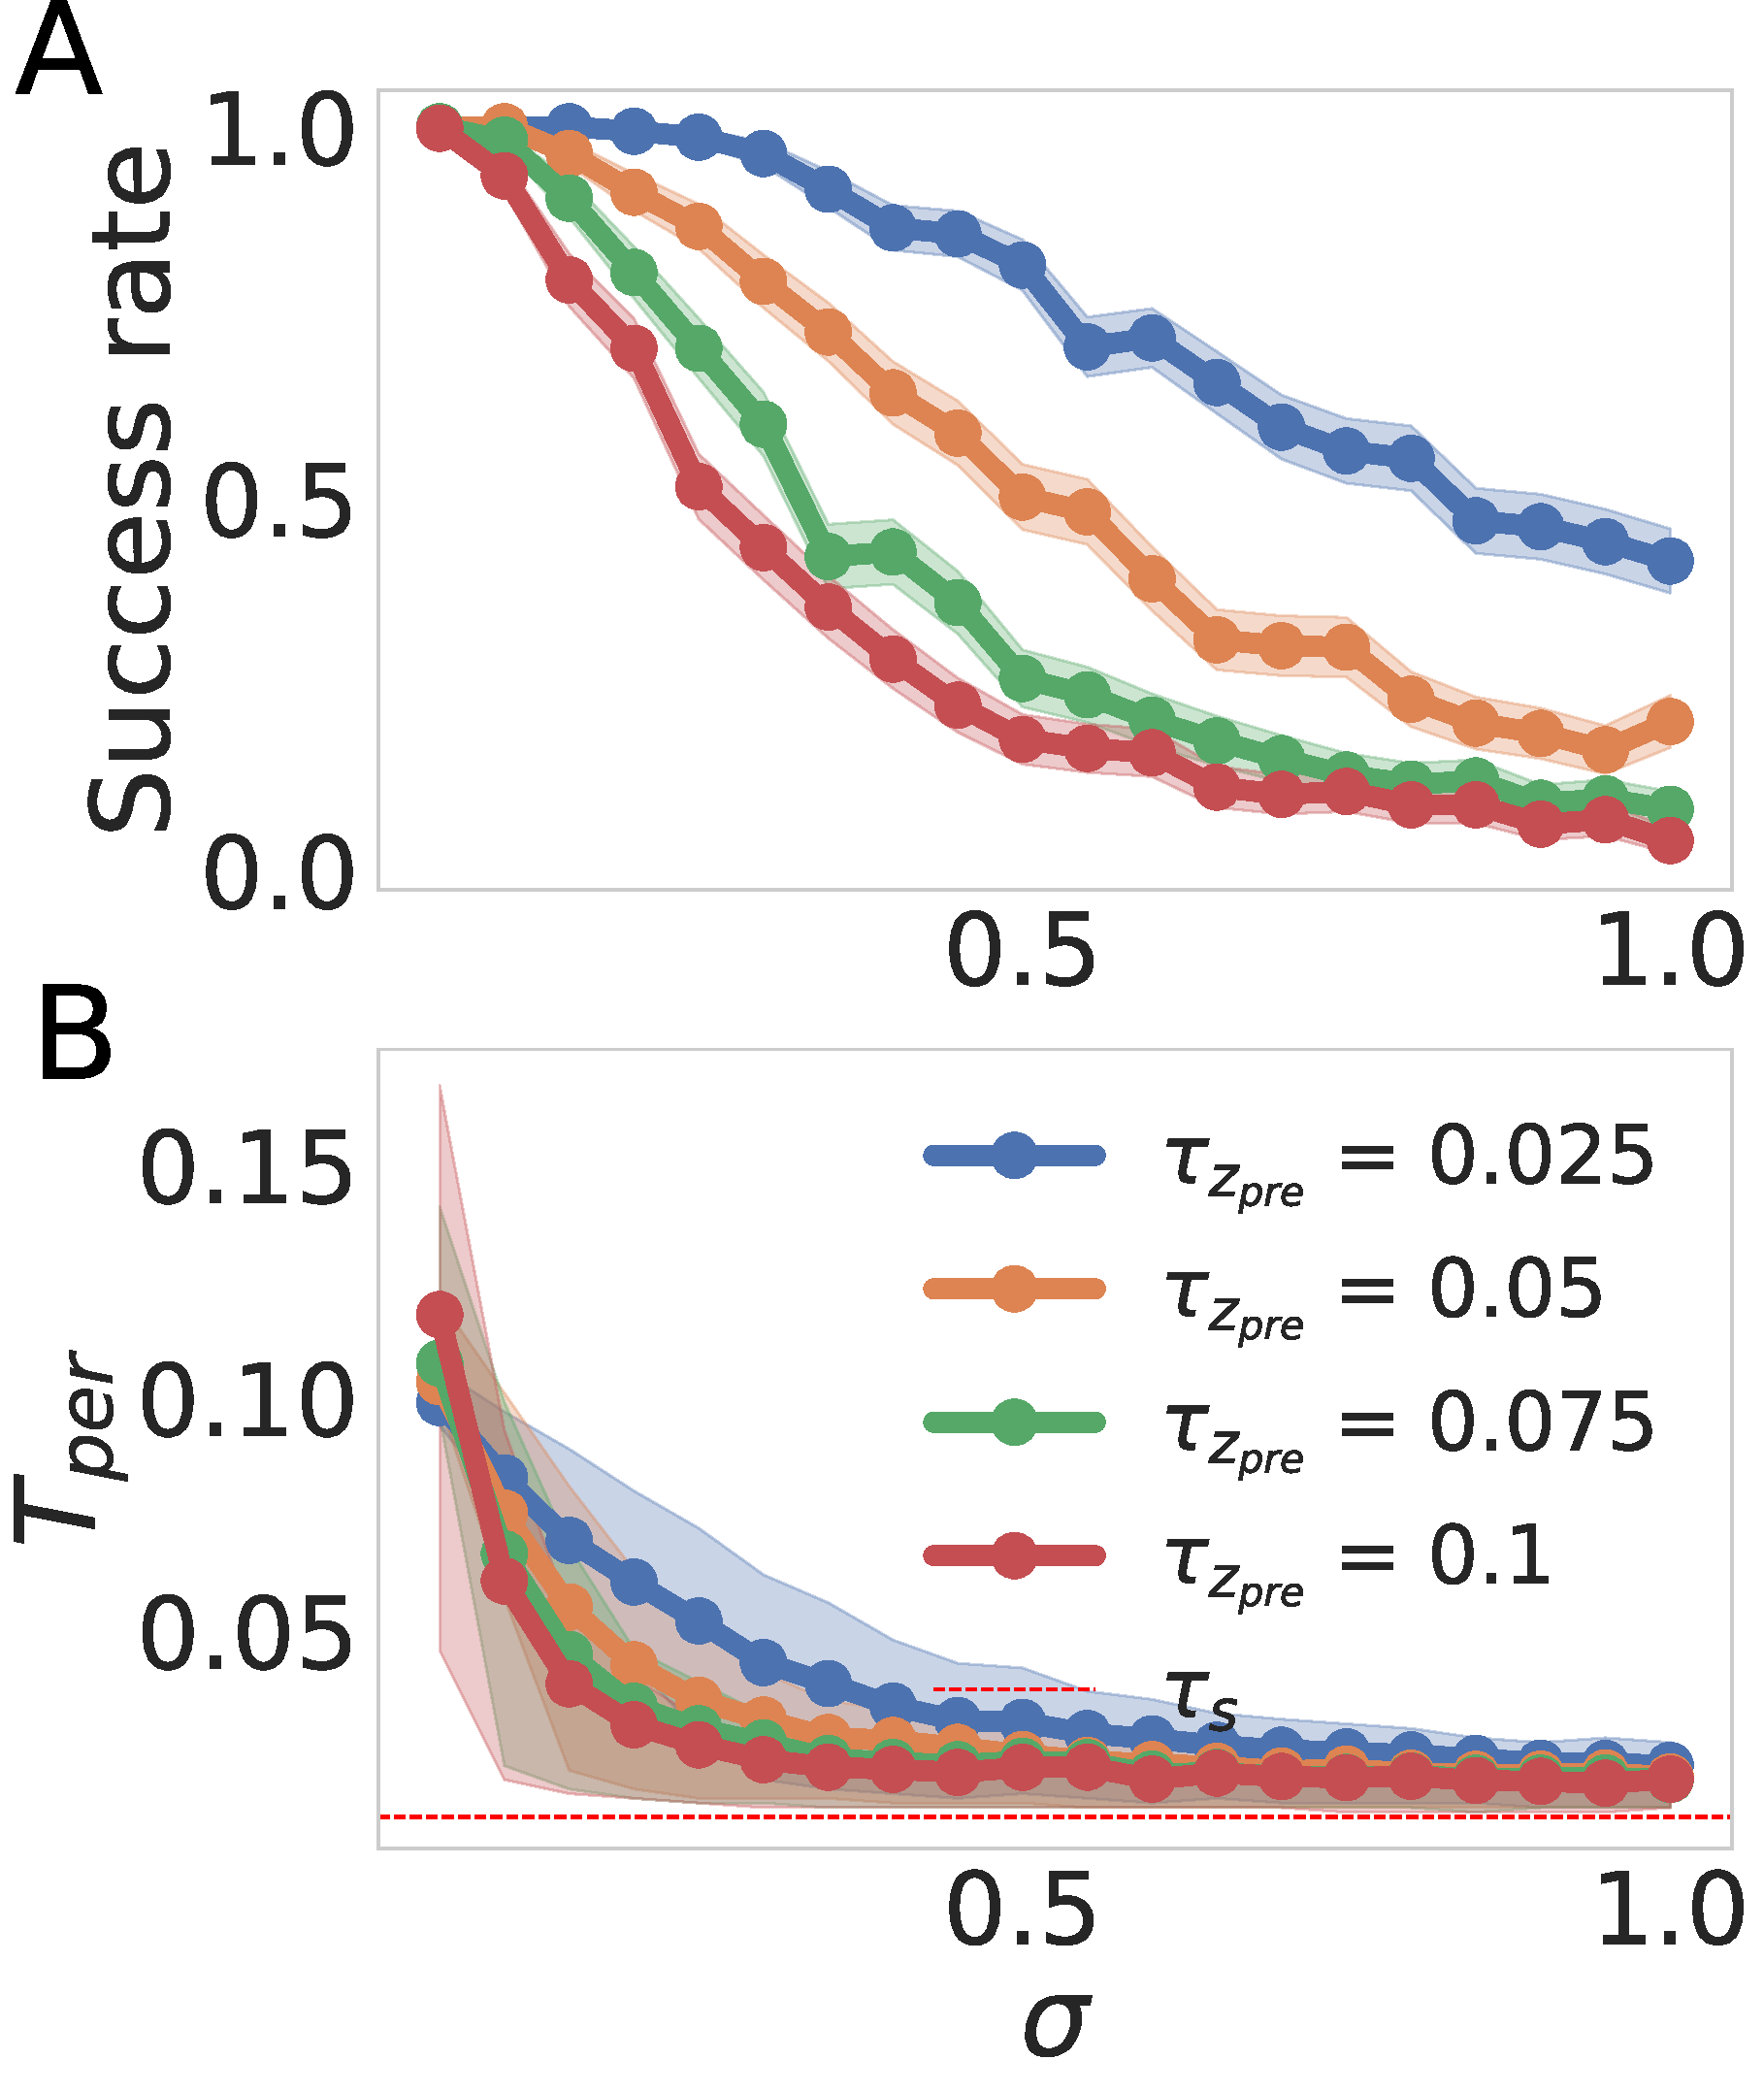
\includegraphics[scale=0.15]{noise_effects.pdf}

\smaller (A) Larger values of the time constant of the synaptic trace ($\tau_{z_{pre}}$) make the system more brittle. (B) The time an attractor remains activated decays in a systematic way in a noisier system. 
\end{center}
 
	
}

%%%%%%%%%%%%%%%%%%%%%%%%%%%%%%%%%%%%%%%%%%%%%%%%%%%%%%%%%%%%%%%%%%%%%%%%%%%%%%
  \headerbox{Sequence disambiguation}{name=disambiguation,column=0,span=1,below=noise}{
%%%%%%%%%%%%%%%%%%%%%%%%%%%%%%%%%%%%%%%%%%%%%%%%%%%%%%%%%%%%%%%%%%%%%%%%%%%%%%
For testing the system disambiguation capabilities we used a framework were we varied the length of a disambiguation window that the system has to overcome.

\begin{center}
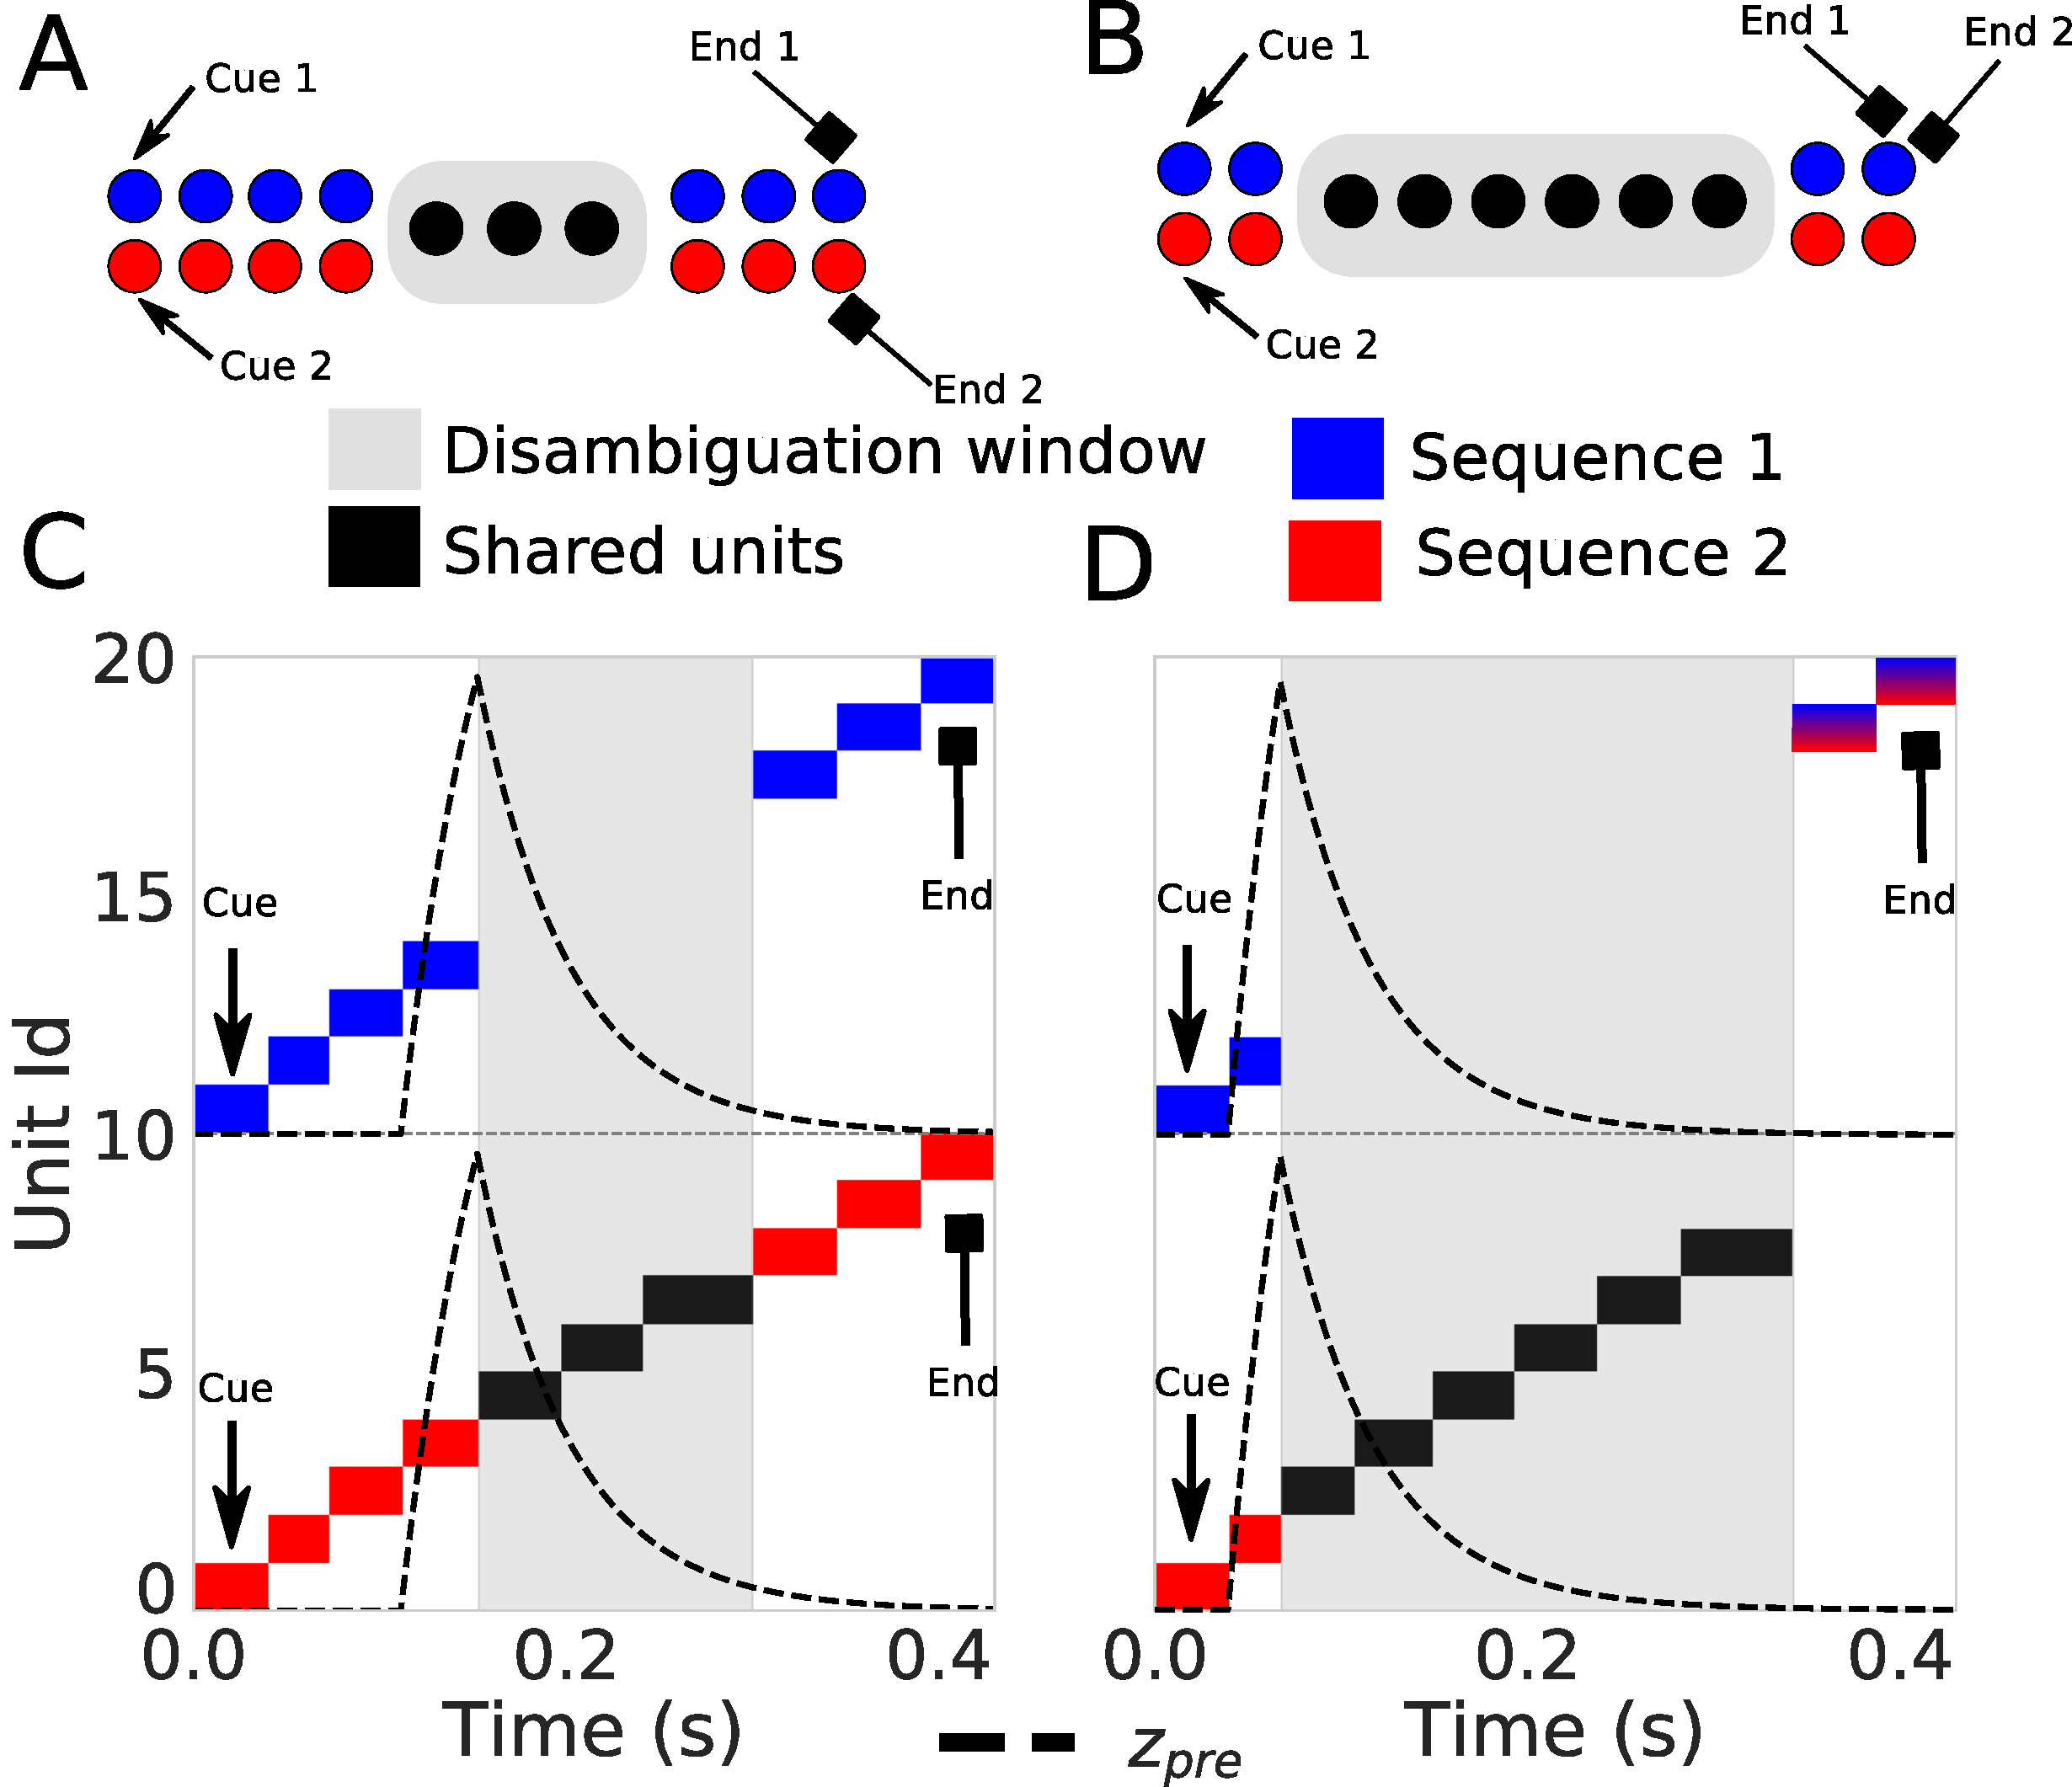
\includegraphics[scale=0.15]{disambiguation_details.pdf}
\smaller (A, B) Schema of a short and long disambiguation windows respectively. (C, D) The synaptic trace preserves the information for long enough to allow disambiguation.  
\end{center}
 
	
}



%%%%%%%%%%%%%%%%%%%%%%%%%%%%%%%%%%%%%%%%%%%%%%%%%%%%%%%%%%%%%%%%%%%%%%%%%%%%%%
  \headerbox{References}{name=references,column=0,above=bottom} {
%%%%%%%%%%%%%%%%%%%%%%%%%%%%%%%%%%%%%%%%%%%%%%%%%%%%%%%%%%%%%%%%%%%%%%%%%%%%%%
    \smaller
    \vspace{-0.4em}
    \bibliographystyle{ieee}
    \renewcommand{\section}[2]{\vskip 0.05em}
      \begin{thebibliography}{1}\itemsep=-0.01em
      \setlength{\baselineskip}{0.4em}
      \bibitem{levy}
      \vspace{5pt}
      Levy, W. B 
      \newblock{579 - 590.}
      \newblock{Hippocampus (1996)}
      \bibitem{phil}
       Tully, Philip J., Henrik Lind\'en, Matthias H. Hennig, and Anders Lansner. 
		\newblock{e1004954.}
        \newblock {\em PLoS Comput Biol 12, no. 5 (2016)}
      \bibitem{anders}
      \vspace{5pt}
        Lansner, Lanserng. and Ekeberg {\"O}rjan
		\newblock{1(01) \: 77 - 87.}
        \newblock {\em International journal of neural systems (1989)}
      \bibitem{us}
      \vspace{5pt}
         Martinez, Ramon Heberto, Pawel Herman, and Anders Lansner
		\newblock{545871}
        \newblock {\em bioRxiv (2019)}
      \end{thebibliography} 
  }


%%%%%%%%%%%%%%%%%%%%%%%%%%%%%%%%%%%%%%%%%%%%%%%%%%%%%%%%%%%%%%%%%%%%%%%%%%%%%%
  \headerbox{The Model}{name=model,column=1,span=2}{
%%%%%%%%%%%%%%%%%%%%%%%%%%%%%%%%%%%%%%%%%%%%%%%%%%%%%%%%%%%%%%%%%%%%%%%%%%%%%%
\begin{multicols}{2}


Based on previous work \cite{phil, us} we present network whose dynamical evolution is controlled by the equations below. The model contains a current $s$ for each unit that evolves according to the their interaction mediated by weights $\mathbf{W}$ and a bias term $\vec{\mathbf{\beta}}$. Furthermore, to induce an structured sequential transition the model is subjected to intrinsic adaptation $\vec{\mathbf{a}}$ and a mechanism of winner-takes-all given by a strict max in $\vec{\mathbf{o}}$. The parameters of the model are given in the table below as well.

\begin{align*}
\tau_s \dfrac{d \vec{s}}{dt} &=  \vec{\mathbf{\beta}} + \mathbf{W} \cdot \vec{\mathbf{z}}_{pre}  - g_a \vec{\mathbf{a}} - \vec{\mathbf{s}}  + \sigma d\vec{\mathbf{\xi}}(t) \\ 
 \tau_a \dfrac{d\vec{\mathbf{a}}}{dt} &= \vec{\mathbf{o}} - \vec{\mathbf{a}} \\ 
o_i &=   \begin{cases}
   1,&  s_i = \underset{hypercolumn}{\max}(\vec{\mathbf{s}}),\\
   0 ,& \text{otherwise}
\end{cases} \\ 
 \tau_{z_{pre}} \dfrac{d\vec{\mathbf{\mathbf{z}}}_{pre}}{dt} &= \vec{\mathbf{o}} - \vec{\mathbf{z}}_{pre} \\ 
\tau_{z_{post}} \dfrac{d \vec{\mathbf{z}}_{post}}{dt} &= \vec{\mathbf{o}} - \vec{\mathbf{z}}_{post} 
\label{eq:dynamics}
\end{align*}

 \begin{center}
    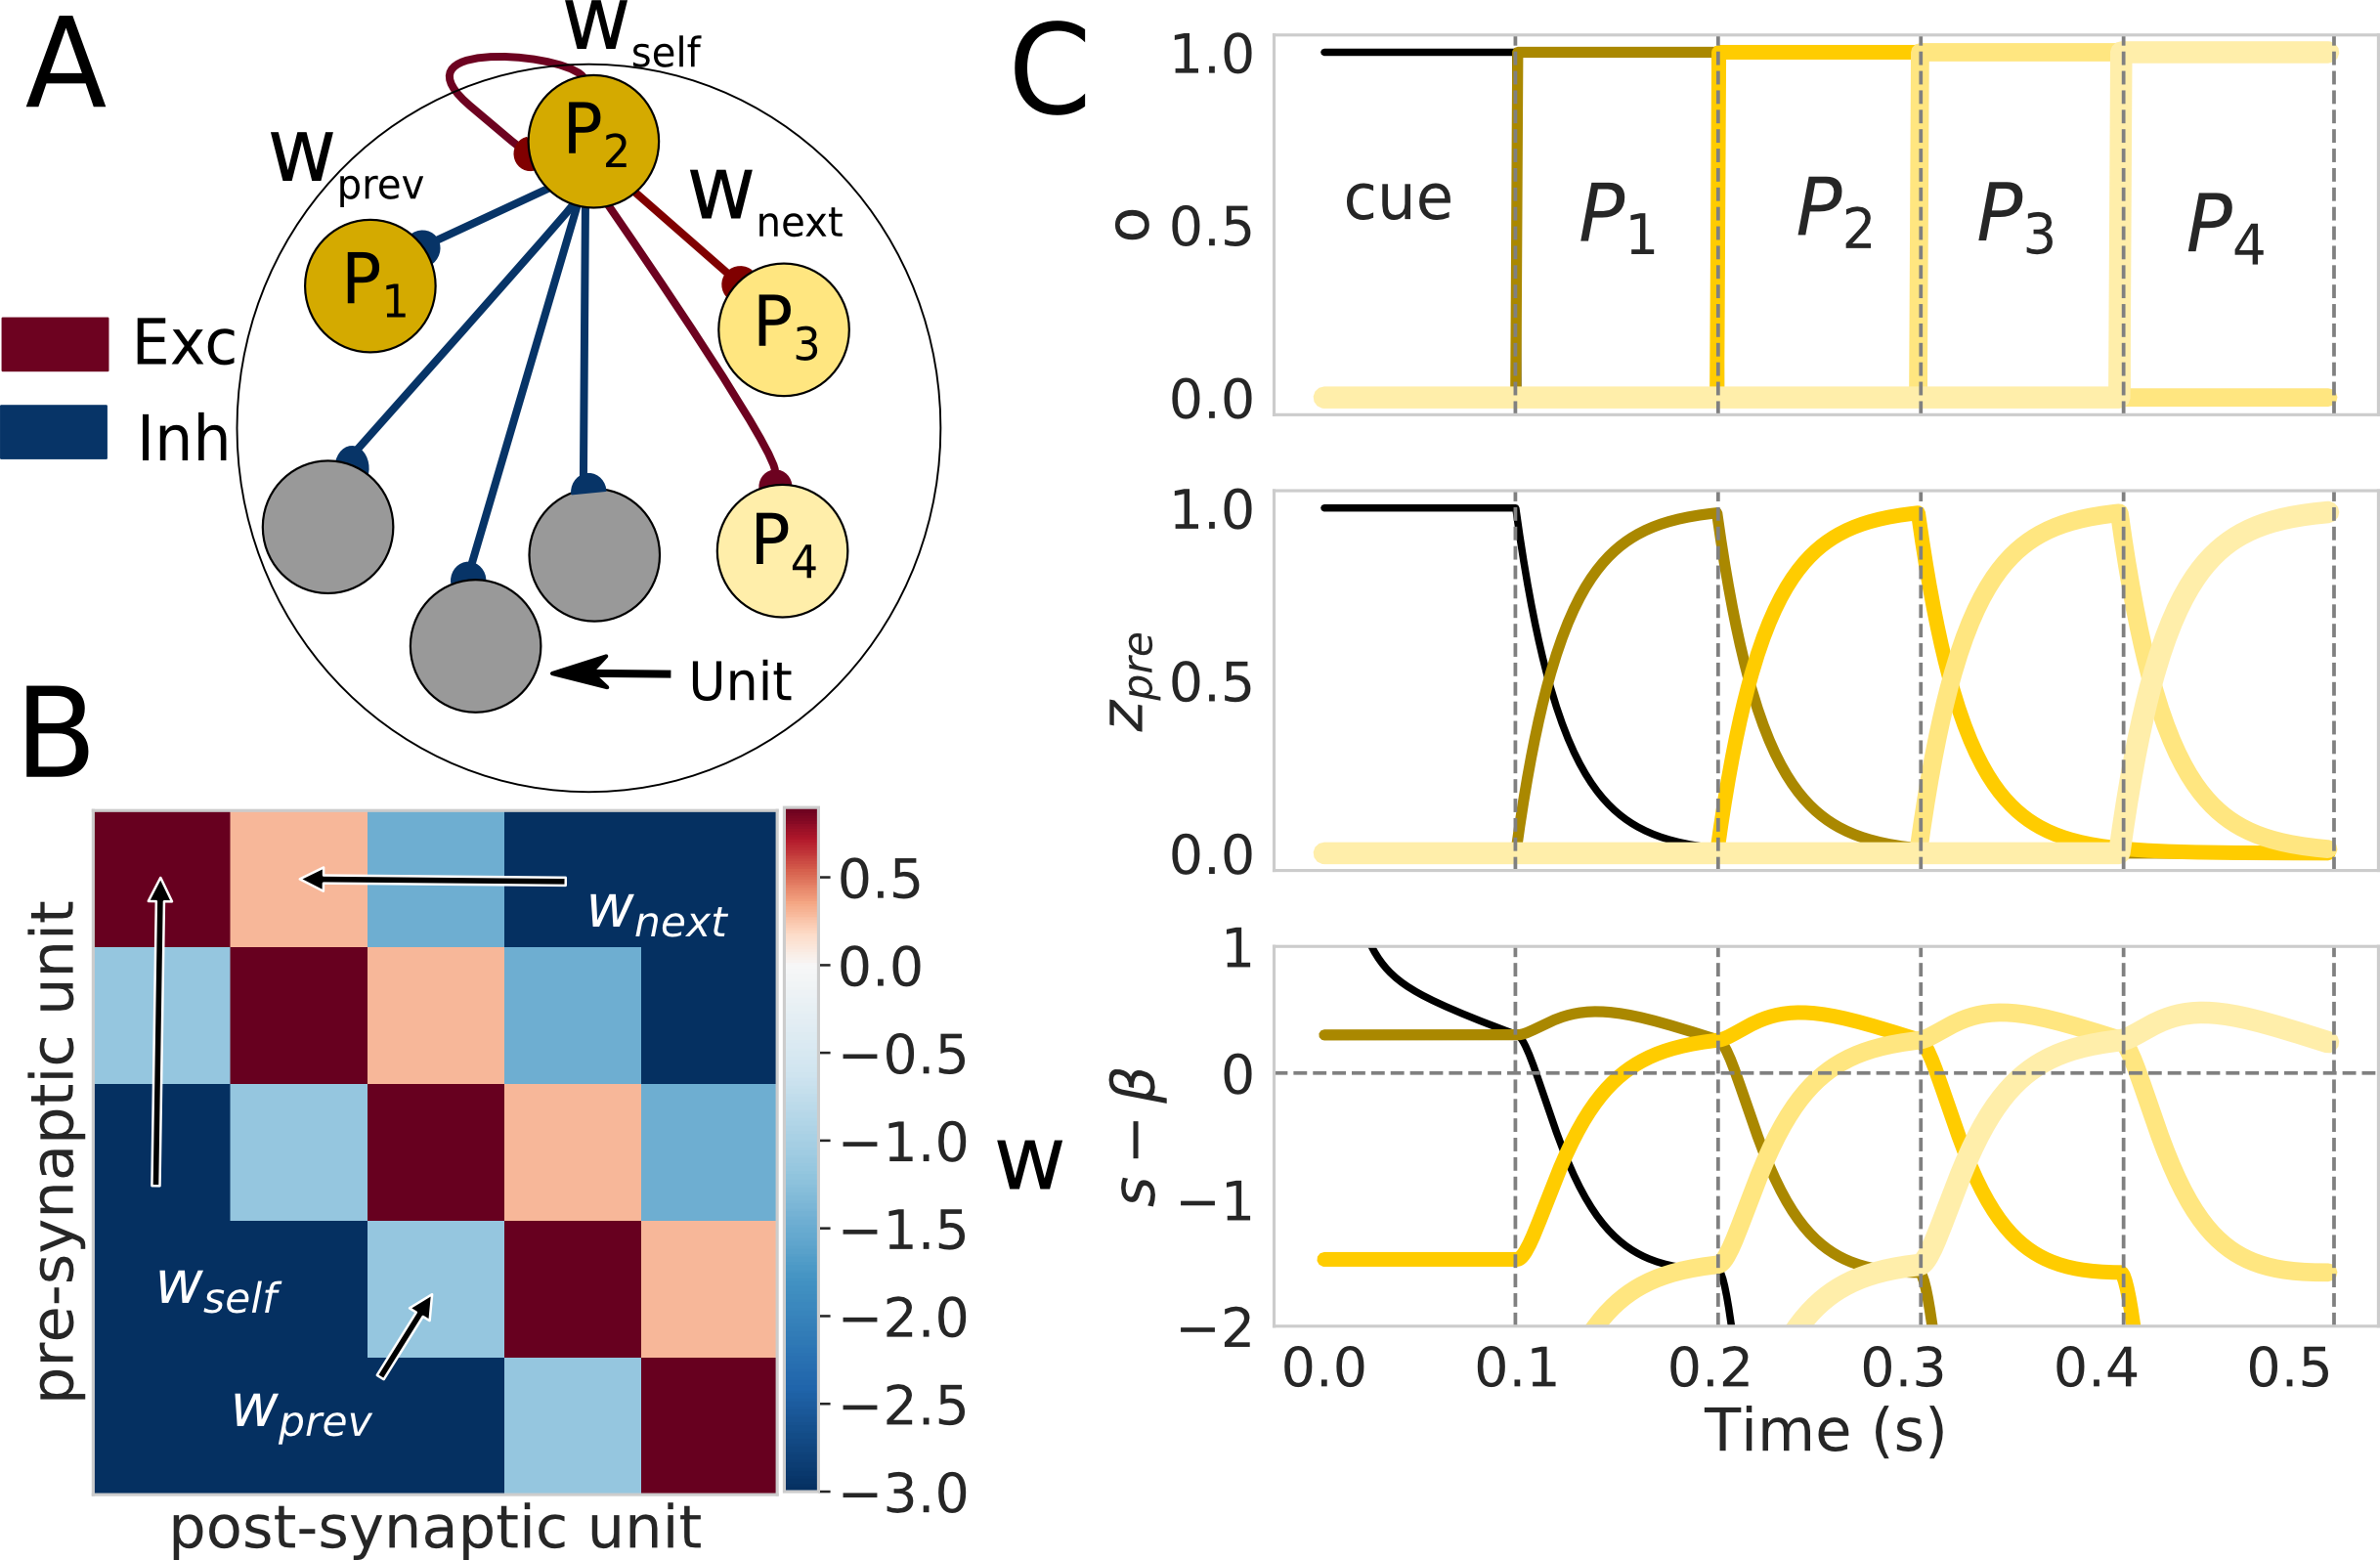
\includegraphics[scale=0.21]{diagram_and_recall.png}
    	\smaller (A) The network. (B) Typical structure of the weight matrix. (C) Recall illustrated with the activity of o, z and the current respectively. 
 \end{center}

As a learning rule we use the Bayesian Confidence Propagator Neural Netowkr (BCPNN) \cite{anders}. The nature of the BCPNN learning rule is such that it connects in an excitatory fashion patterns that more often that not appear together (in a probabilistic sense) and connects in an inhibitory fashion patterns that do not. More importantly for sequence disambiguation the BCPNN automatically accounts for balanced connections in sequential forks. 

\begin{align*}
t \dfrac{d \vec{\mathbf{p}}_{pre}}{dt} &= \vec{\mathbf{z}}_{pre} - \vec{\mathbf{p}}_{pre}  
 \\
 t\dfrac{d\mathbf{P}}{dt} &= \vec{\mathbf{p}}_{pre} \otimes \vec{\mathbf{p}}_{post} -\mathbf{P}  \\ 
 t\dfrac{d\vec{\mathbf{p}}_{post}}{dt} &= \vec{\mathbf{z}}_{post} - \vec{\mathbf{p}}_{post}  \\
 \mathbf{W} &= \log \left(\frac{\mathbf{P}}{\vec{\mathbf{p}}_{pre} \otimes \vec{\mathbf{p}}_{post}} \right)  \\ 
 \vec{\mathbf{\beta}} &= \log \left( \vec{\mathbf{p}}_{post}  \right) 
\end{align*}

  \begin{center}
    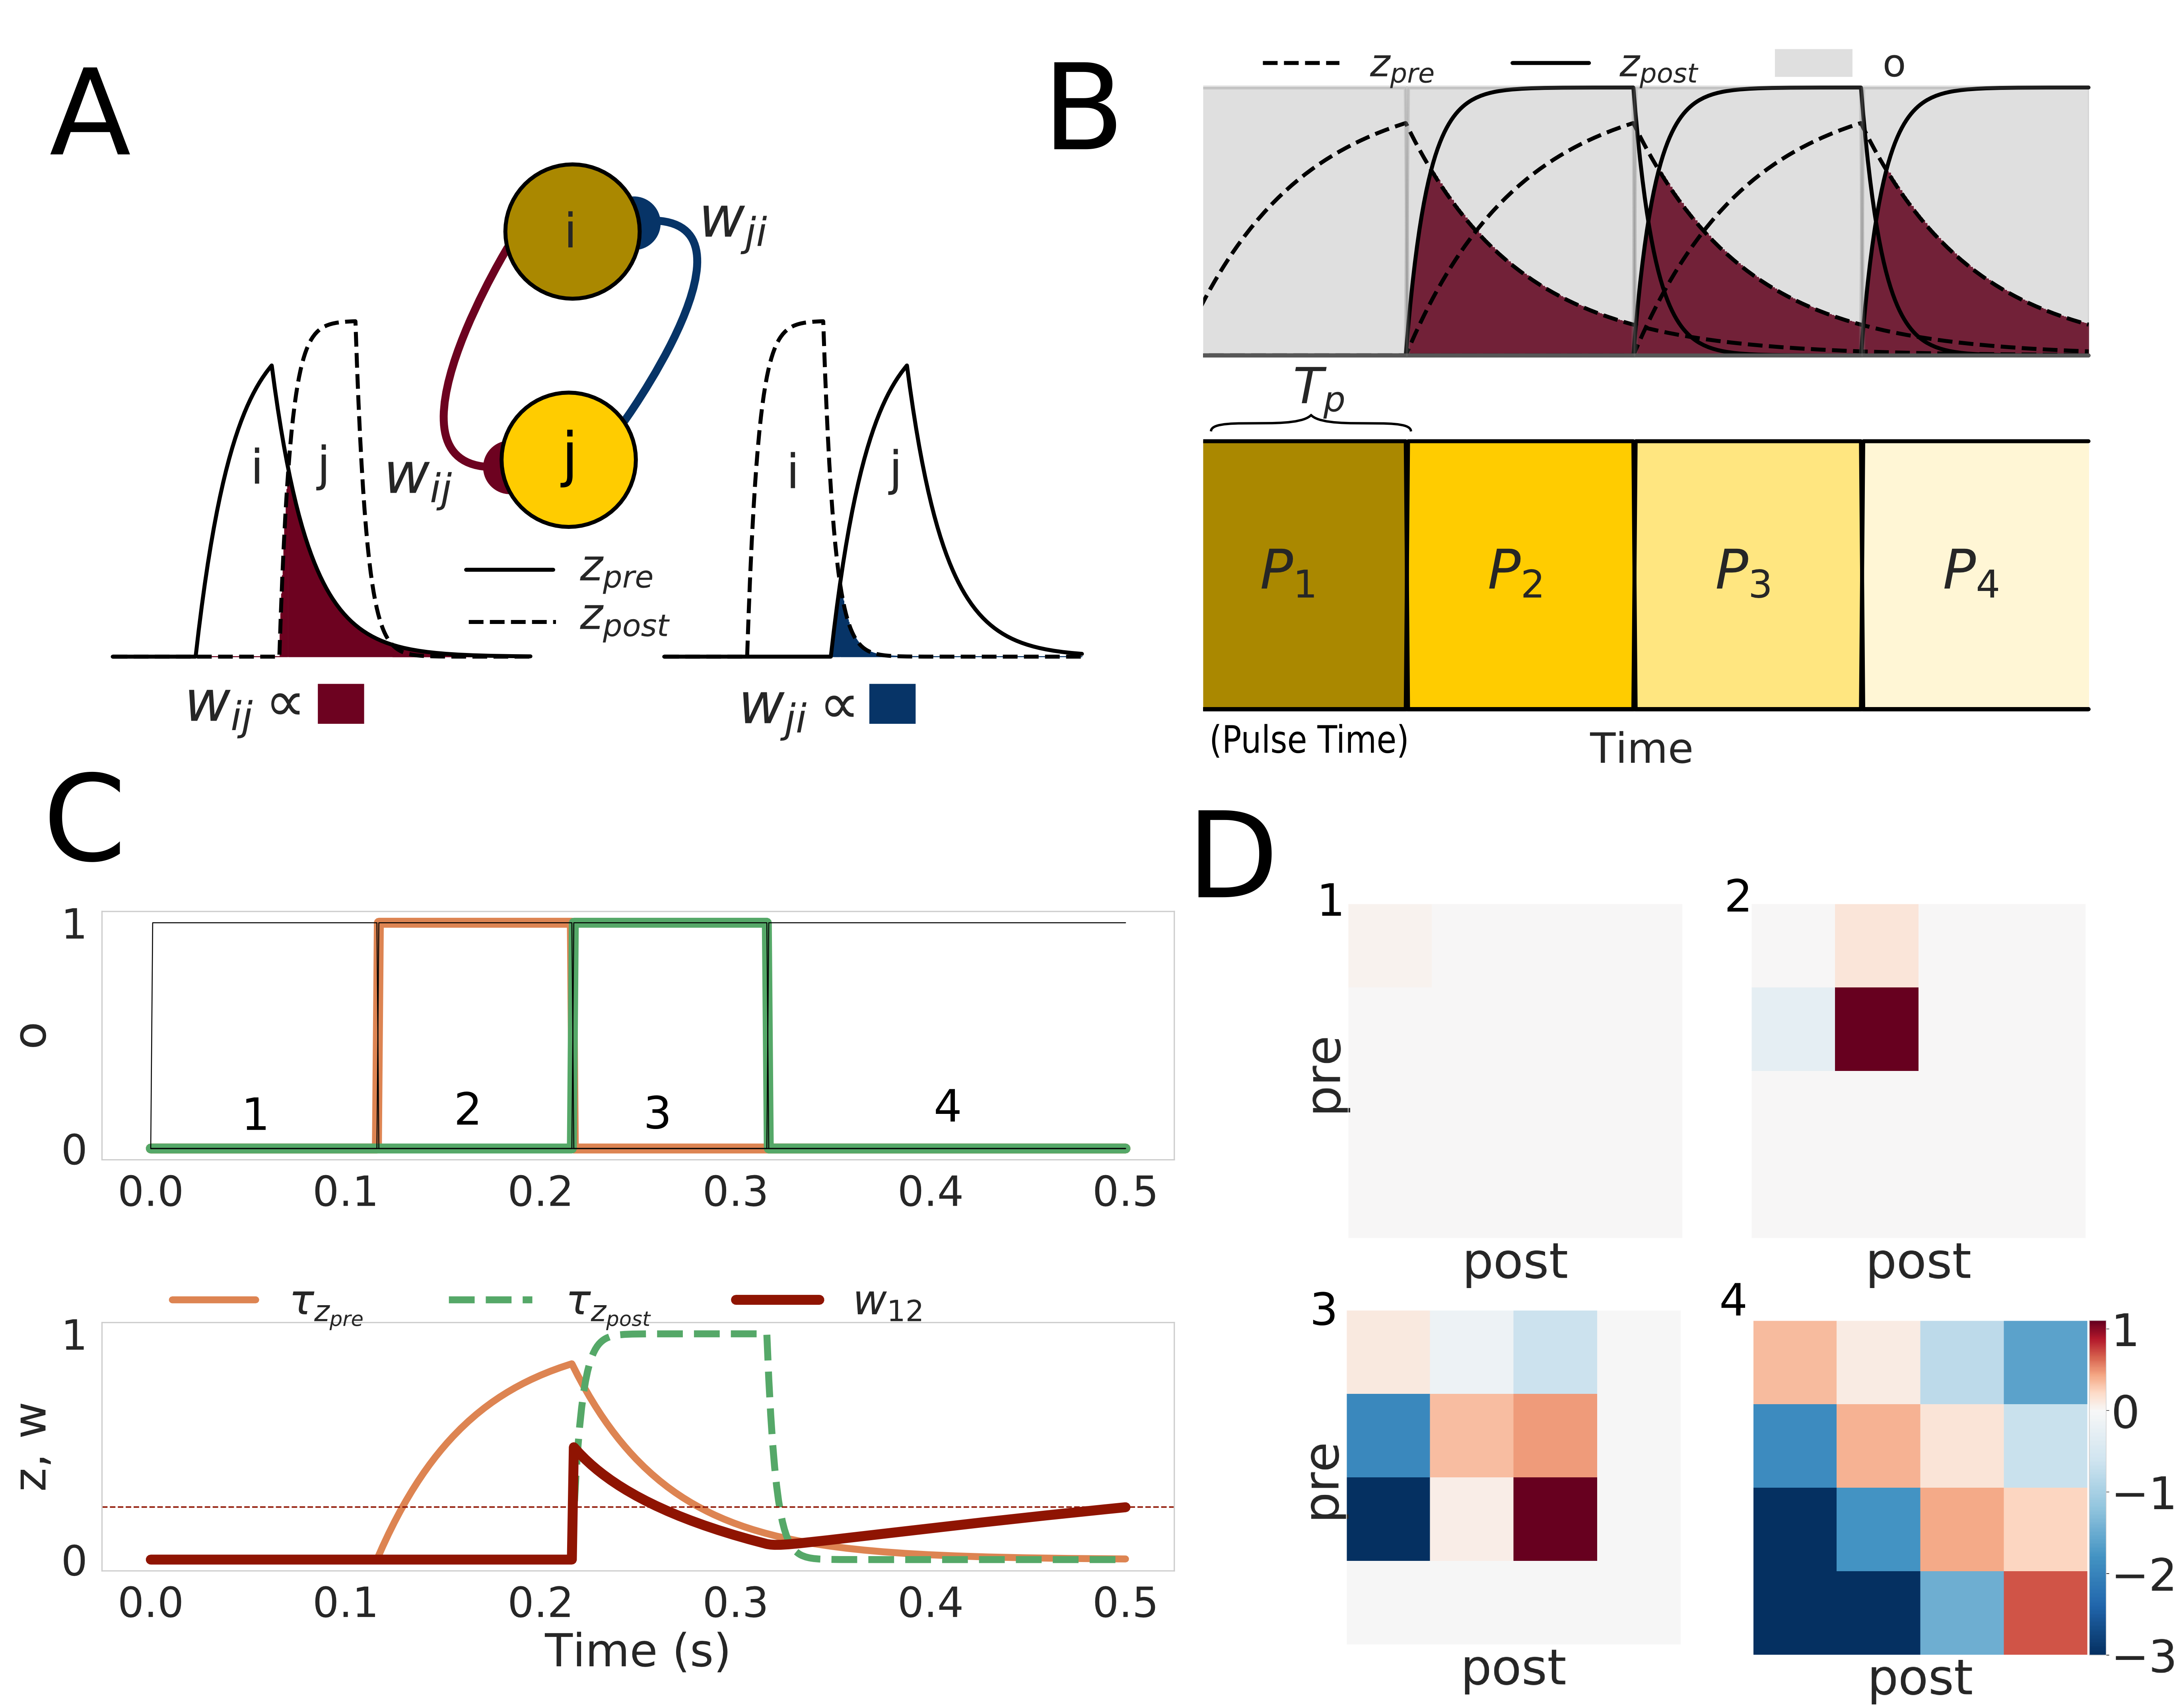
\includegraphics[scale=0.10]{learning.png}
	\smaller (A) Illustration of the learning rule. (B) The training protocol. (C) Weight evolution responds to coincidences in time. (D) Evolution of the weight matrix as patterns are presented to the network.  
  \end{center}
  

  \resizebox{\linewidth}{!}{
\begin{tabular}{|c|c|c|}
\toprule
Symbol            & Name                                  & Values          \\ \midrule
$\tau_s$          & Synaptic time constant                & $10 \: ms$      \\
$\tau_a$          & Adaptation time constant              & $250 \: ms$     \\
$g_a$             & Adaptation gain                       & $0 - 2.5$  (units of $w$, control) \\
$\tau_{z_{pre}}$  & Pre synaptic z-filter time constant   & $5 - 150 \: ms$ \\
$\tau_{z_{post}}$ & Post synaptic z-filter time constant  & $5 \: ms$       \\
$\tau_p$          & Probability traces time constant       & $5 \: s$       \\
$\sigma$          & Standard deviation of s values        & $0 - 3$        \\
$T_{per}$         & Persistence time                      & $50-3000 \: ms$ (controlled)      \\
$T_{p}$           & Pulse time                            & $100 \: ms$     \\ 
$\Delta T_{p}$    & Inter Pulse Interval (IPI)            & $0 \: ms$       \\ \bottomrule
\end{tabular}
}

 \begin{center}
\smaller Typical parameter's values. 
\end{center}
\end{multicols}

  }



%%%%%%%%%%%%%%%%%%%%%%%%%%%%%%%%%%%%%%%%%%%%%%%%%%%%%%%%%%%%%%%%%%%%%%%%%%%%%%%
\headerbox{Results}{name=tau, column=1,span=2, below=model}{
%%%%%%%%%%%%%%%%%%%%%%%%%%%%%%%%%%%%%%%%%%%%%%%%%%%%%%%%%%%%%%%%%%%%%%%%%%%%%%%

We tested the disambiguation power of the system for different arrangements of the synaptic trace time constant ($\tau_{z_{pre}}$), disambiguation windows and three noise regimes: small ($\sigma = 0.05$), medium ($\sigma=0.1$) and large ($\sigma=0.15$).  

\begin{multicols}{2}
\begin{center}
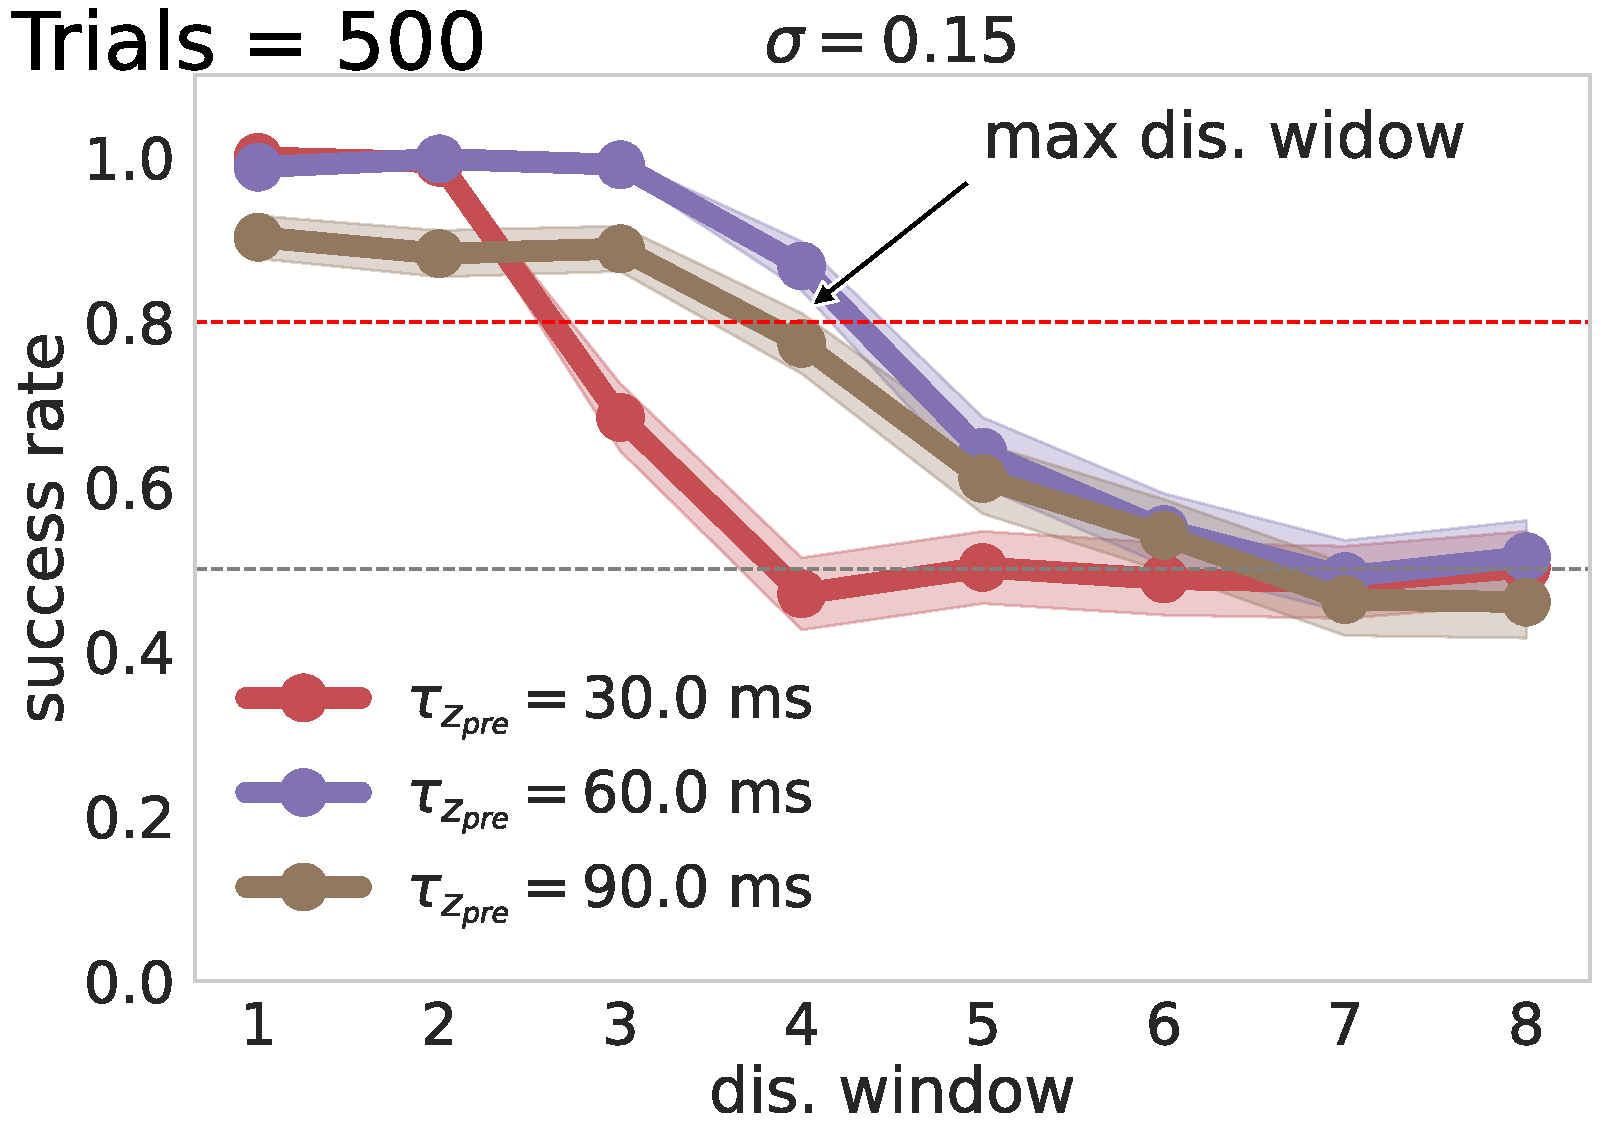
\includegraphics[scale=0.20]{noise2.pdf}

\smaller Success rate as a function of the disambiguation window length for different values of $\tau_{z_{pre}}$.
\end{center}

\begin{center}
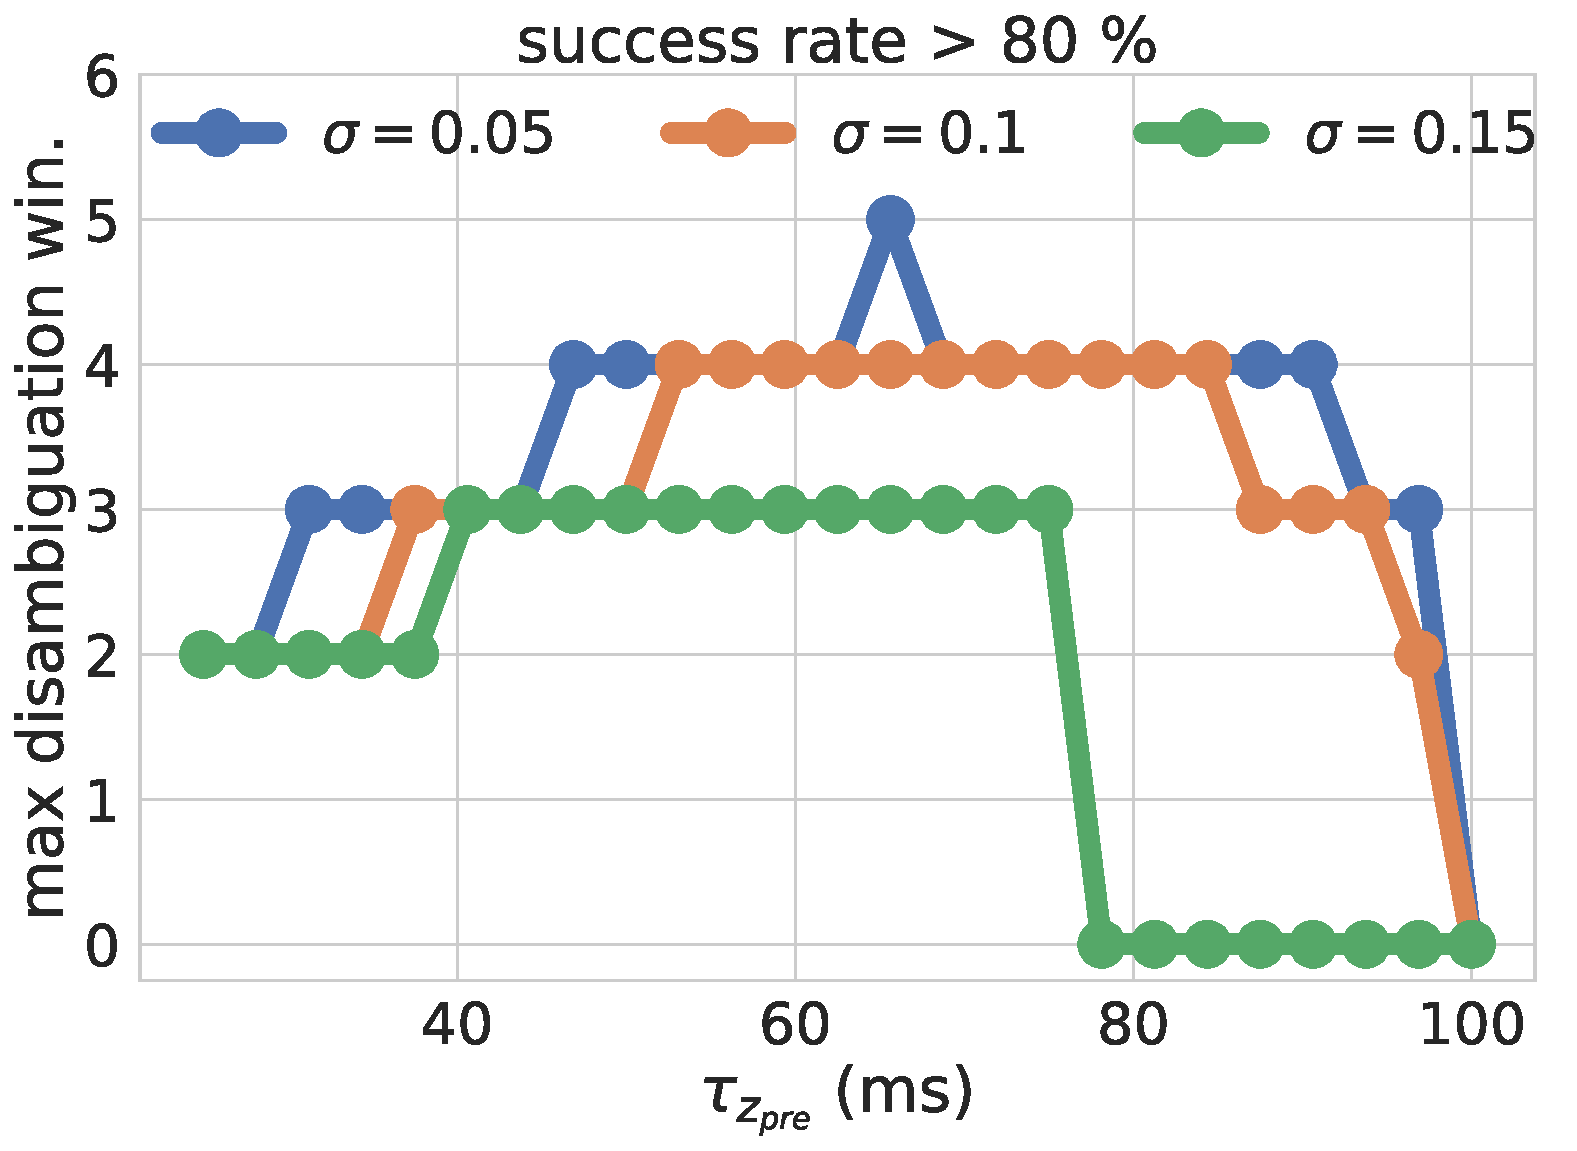
\includegraphics[scale=0.20]{noise.pdf}

\smaller Max disambiguation window depending as a function of $\tau_{z_{pre}}$ in different noise regimes. 
\end{center}

\end{multicols}


}



%%%%%%%%%%%%%%%%%%%%%%%%%%%%%%%%%%%%%%%%%%%%%%%%%%%%%%%%%%%%%%%%%%%%%%%%%%%%%%%
\headerbox{Funding}{name=funding,column=1,span=2,above=bottom}{
%%%%%%%%%%%%%%%%%%%%%%%%%%%%%%%%%%%%%%%%%%%%%%%%%%%%%%%%%%%%%%%%%%%%%%%%%%%%%%%
\begin{multicols}{2} 
 
 \smaller 
  \hspace{1em} This work was supported by the Erasmus Mundus Joint Doctoral Program Eurospin. 
  
 
\begin{center}

\includegraphics[height=6em]{logo_em.png}
\end{center}

\end{multicols}

}




\end{poster}%
\end{document}
